\documentclass[11pt,a4paper]{article}

\usepackage[utf8]{inputenc}
\usepackage[T1]{fontenc}
\usepackage[margin=2.3cm]{geometry}
\usepackage{amsmath,amssymb,bm}
\usepackage{graphicx}
\usepackage{subcaption}
\usepackage{booktabs}
\usepackage{listings}
\usepackage{xcolor}
\usepackage{float}
\usepackage[hidelinks]{hyperref}

\lstset{
  language=Python,
  basicstyle=\ttfamily\footnotesize,
  keywordstyle=\color{blue!60!black}\bfseries,
  commentstyle=\color{green!40!black},
  stringstyle=\color{red!50!black},
  frame=single,
  breaklines=true,
  columns=fullflexible,
  showstringspaces=false
}

\title{Reinforcement Learning WS 2026/27\\Homework Sheet 6}
\author{Anna Notaro 7624771, Maximilian Hemmann 7627178, Jan Hischke 7600876}
\date{\today}

\begin{document}
\maketitle

%======================================================================
\section{Score Function for a Gaussian Policy}

The policy is
\[
  \pi_\theta(s,a) = \frac{1}{\sigma\sqrt{2\pi}}
  \exp\!\left(-\frac{(a-\mu(s,\theta))^2}{2\sigma^2}\right),
  \qquad \mu(s,\theta) = \phi(s)^\top\theta .
\]

\paragraph{(a)} Taking the logarithm gives
\[
  \log \pi_\theta(s,a) = -\log\!\left(\sigma\sqrt{2\pi}\right)
  - \frac{\left(a-\phi(s)^\top\theta\right)^2}{2\sigma^2}.
\]
The first term does not depend on $\theta$. With the chain rule and
$\nabla_\theta\, \phi(s)^\top\theta = \phi(s)$ we get
\[
  \nabla_\theta \log \pi_\theta(s,a)
  = -\frac{1}{2\sigma^2}\cdot 2\left(a-\phi(s)^\top\theta\right)\cdot\left(-\phi(s)\right)
  = \boxed{\frac{1}{\sigma^2}\left(a-\phi(s)^\top\theta\right)\phi(s)} .
\]
The score points in the direction of the feature vector. It is scaled by how
far the sampled action lies from the mean, relative to the variance: actions
above the mean push $\mu$ up, and actions below it push $\mu$ down.

%======================================================================
\section{Deep Q-Learning}

%----------------------------------------------------------------------
\subsection*{(b), (c) Pendulum-v1}

\begin{table}[H]
  \centering
  \begin{tabular}{lrr}
    \toprule
    Variant & Mean return & Std \\
    \midrule
    No target network                         & $-170.00$ & $100.46$ \\
    Target net updated every training call    & $-141.24$ & $87.12$  \\
    Target net updated every 20 training calls& $-245.74$ & $594.84$ \\
    \bottomrule
  \end{tabular}
  \caption{Pendulum-v1: test return after 600 training episodes (50 greedy
  episodes). Updating the target network every training call works best. The
  large std for $k=20$ comes from 1--2 test episodes in which the pendulum never
  swings up.}
  \label{tab:pendulum}
\end{table}

\begin{figure}[H]
  \centering
  \begin{subfigure}{0.32\textwidth}
    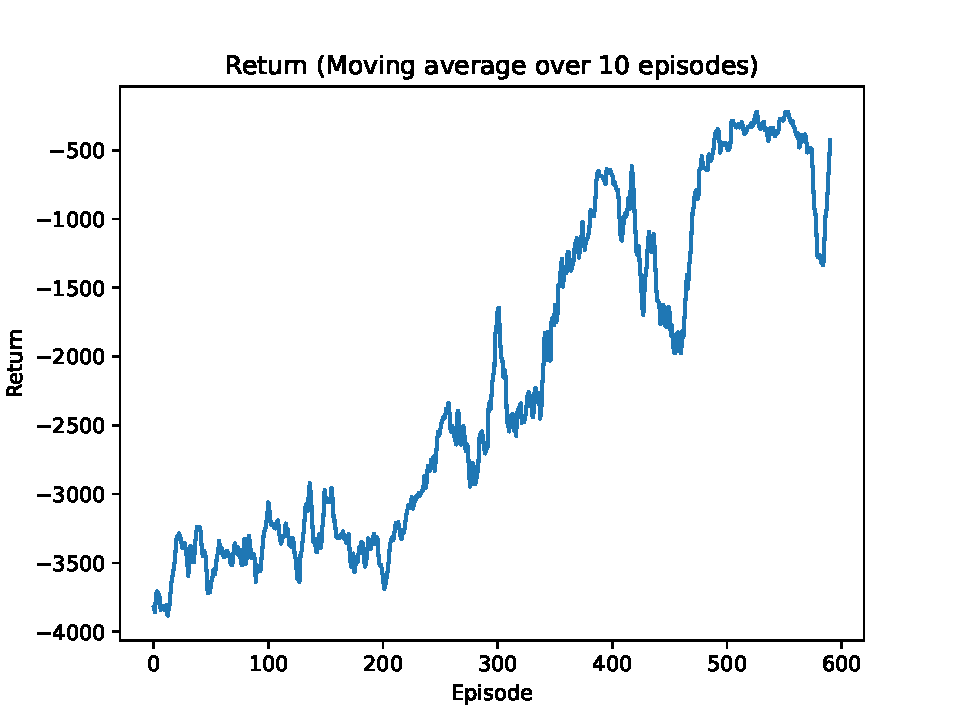
\includegraphics[width=\linewidth]{figures/pendulum/return_train_no_target_network.pdf}
    \caption{No target network}
  \end{subfigure}
  \begin{subfigure}{0.32\textwidth}
    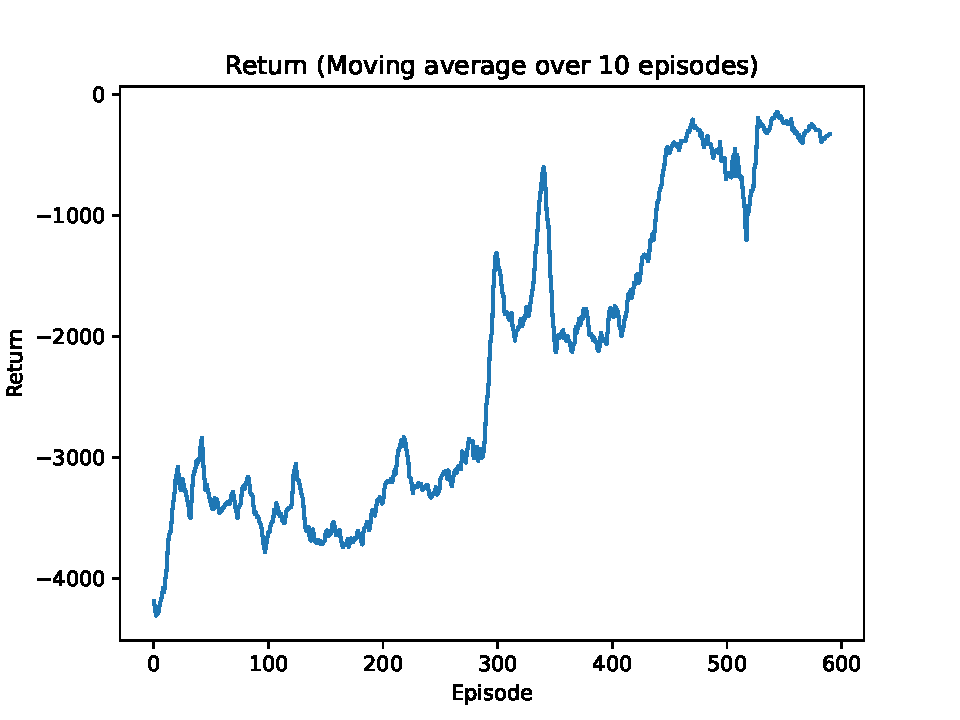
\includegraphics[width=\linewidth]{figures/pendulum/return_train_update_every_call.pdf}
    \caption{Update every call}
  \end{subfigure}
  \begin{subfigure}{0.32\textwidth}
    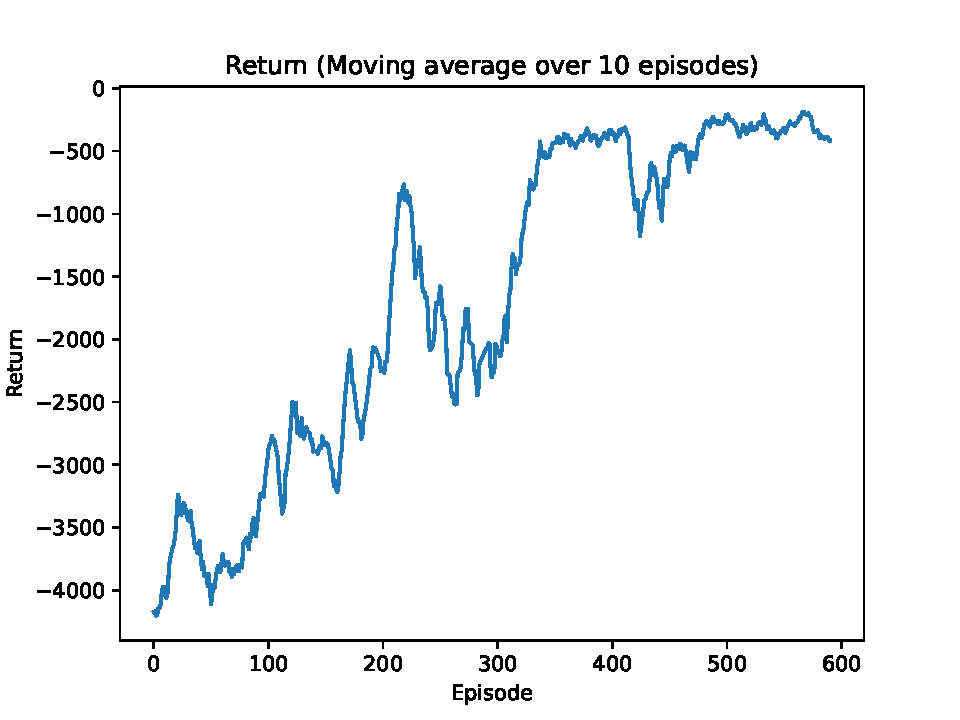
\includegraphics[width=\linewidth]{figures/pendulum/return_train_update_every_20_calls.pdf}
    \caption{Update every 20 calls}
  \end{subfigure}
  \caption{Pendulum-v1: training return (running mean over 10 episodes). All
  three variants learn to swing up the pendulum, and the return rises from
  about $-4000$ to a few hundred.}
  \label{fig:pend-return}
\end{figure}

\begin{figure}[H]
  \centering
  \begin{subfigure}{0.32\textwidth}
    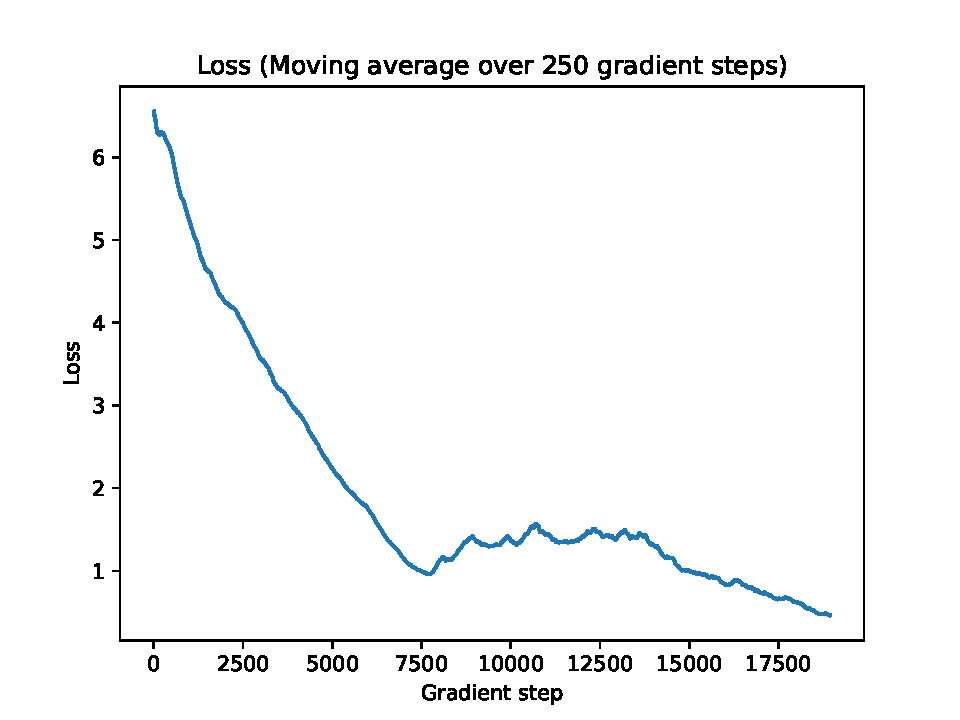
\includegraphics[width=\linewidth]{figures/pendulum/loss_train_no_target_network.pdf}
    \caption{No target network}
  \end{subfigure}
  \begin{subfigure}{0.32\textwidth}
    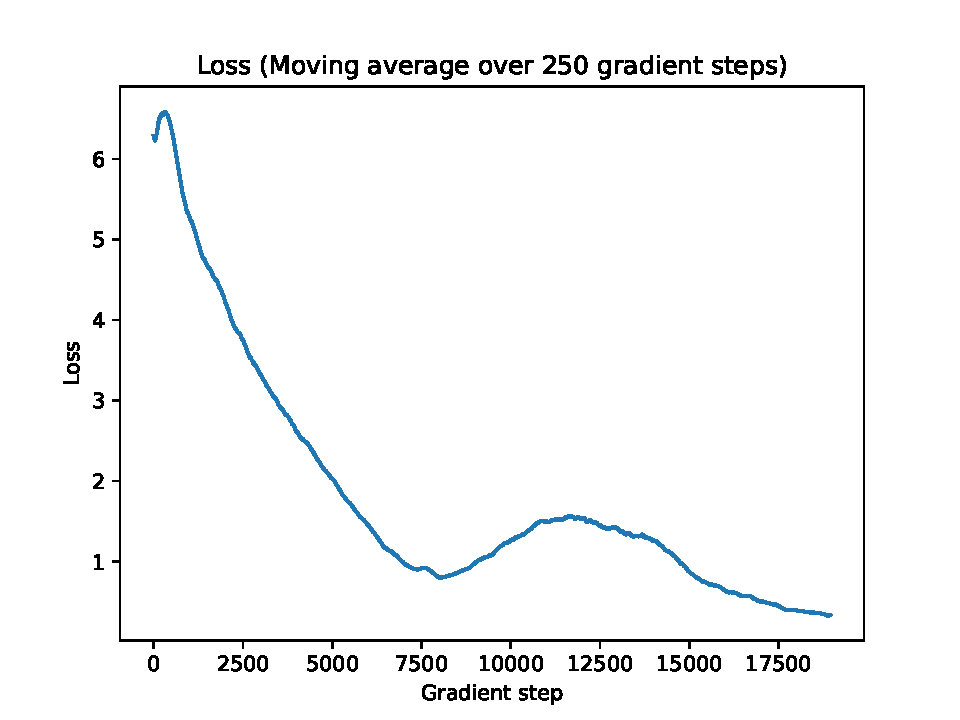
\includegraphics[width=\linewidth]{figures/pendulum/loss_train_update_every_call.pdf}
    \caption{Update every call}
  \end{subfigure}
  \begin{subfigure}{0.32\textwidth}
    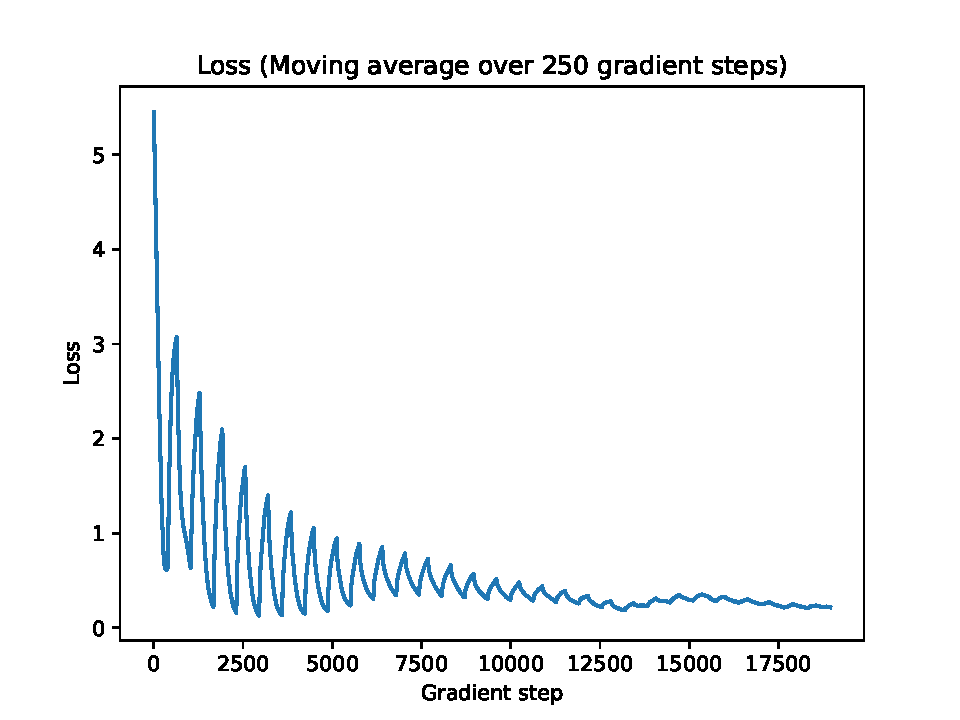
\includegraphics[width=\linewidth]{figures/pendulum/loss_train_update_every_20_calls.pdf}
    \caption{Update every 20 calls}
  \end{subfigure}
  \caption{Pendulum-v1: training loss (running mean over 250 gradient steps).
  With $k=20$ the loss has a saw-tooth shape: it falls while the targets are
  fixed and jumps whenever the target network is replaced.}
  \label{fig:pend-loss}
\end{figure}

%----------------------------------------------------------------------
\subsection*{(d) Value function}

\begin{figure}[H]
  \centering
  \begin{subfigure}{0.32\textwidth}
    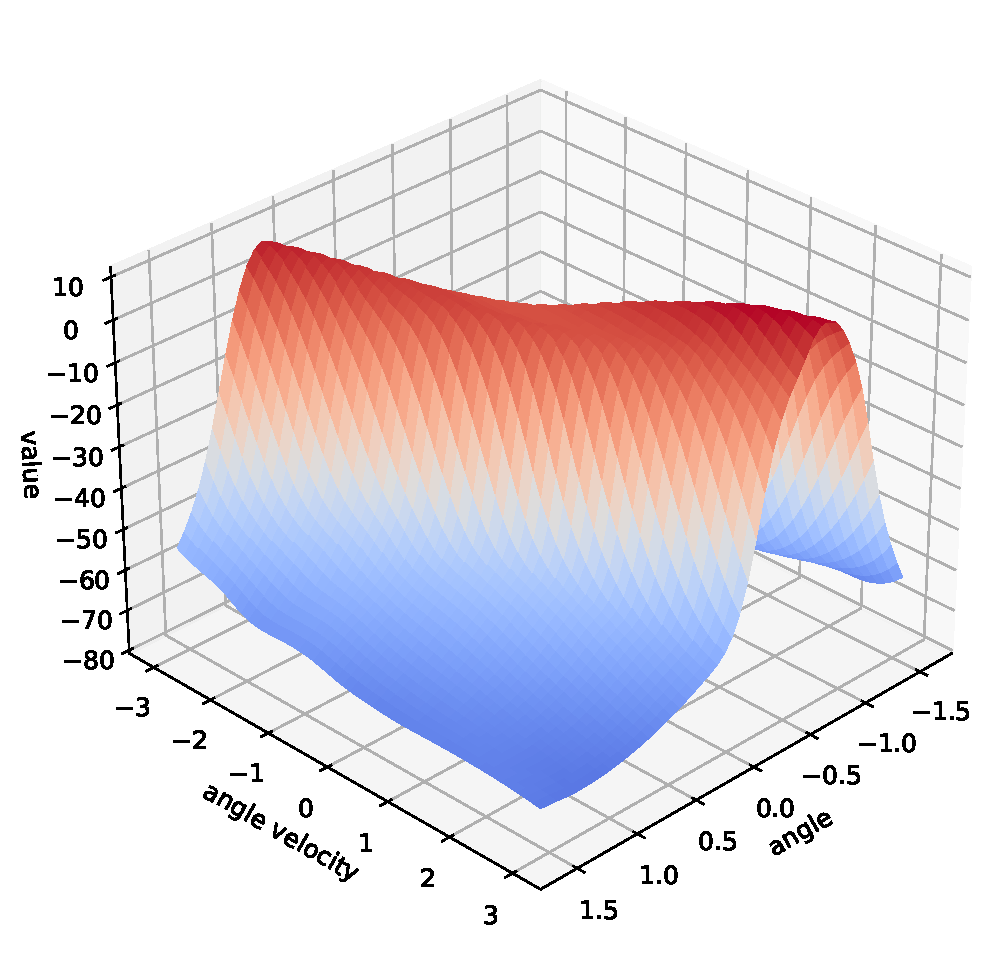
\includegraphics[width=\linewidth]{figures/pendulum/value_function_no_target_network.pdf}
    \caption{No target network}
  \end{subfigure}
  \begin{subfigure}{0.32\textwidth}
    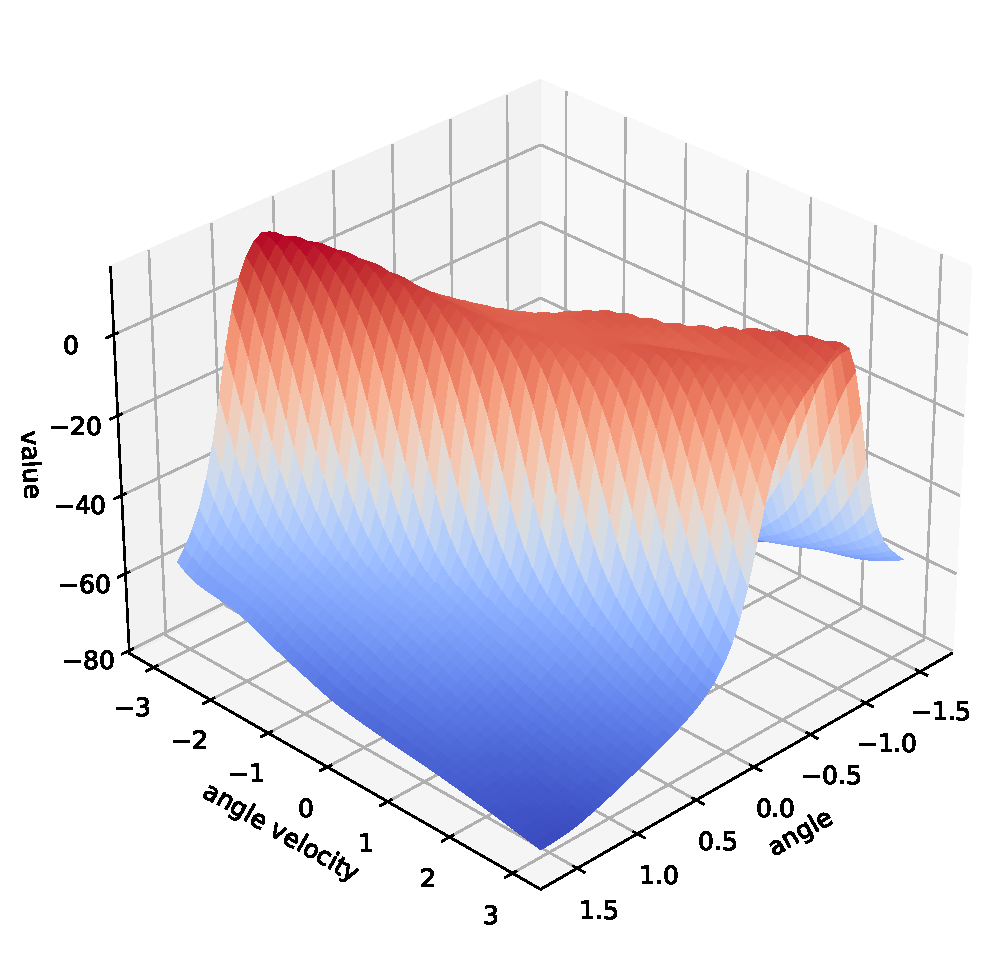
\includegraphics[width=\linewidth]{figures/pendulum/value_function_update_every_call.pdf}
    \caption{Update every call}
  \end{subfigure}
  \begin{subfigure}{0.32\textwidth}
    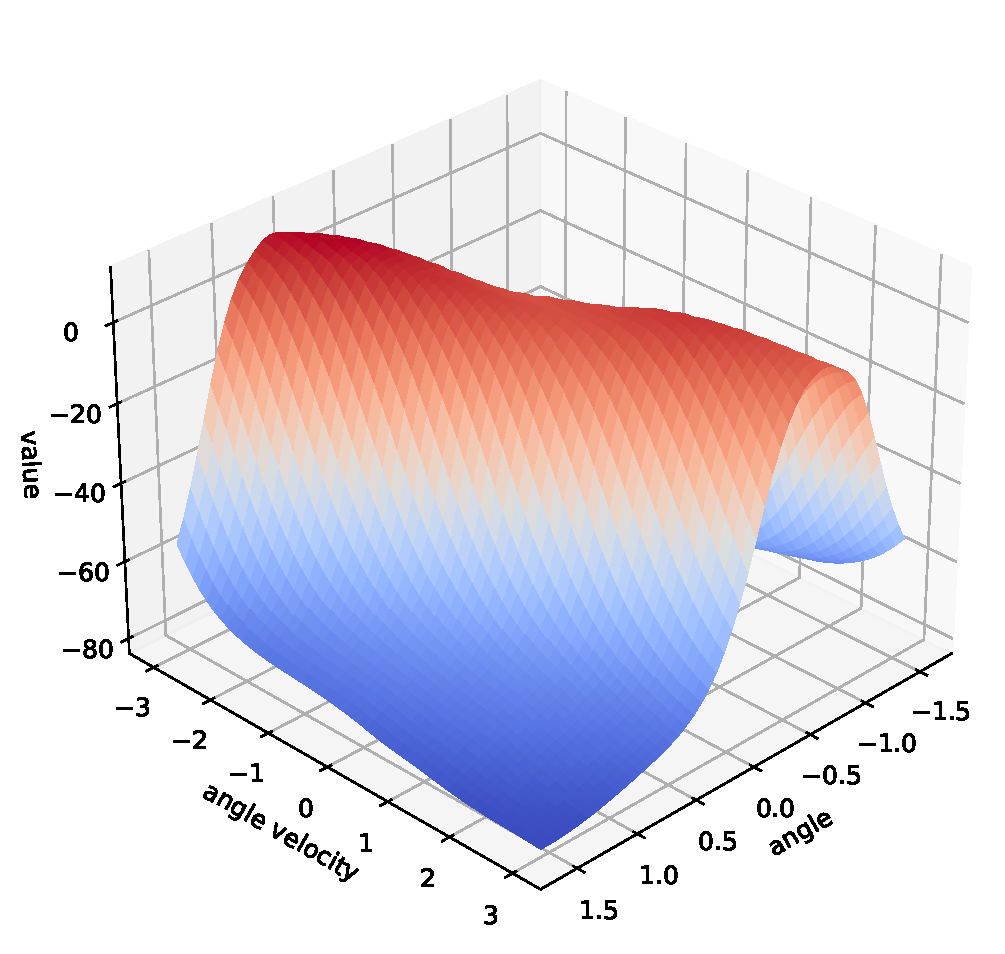
\includegraphics[width=\linewidth]{figures/pendulum/value_function_update_every_20_calls.pdf}
    \caption{Update every 20 calls}
  \end{subfigure}
  \caption{Pendulum-v1: $\max_a Q(s,a)$ over angle (0 = upright) and angular
  velocity. The value is highest near the upright position and when the
  pendulum moves back towards it. It is lowest where angle and velocity have
  the same sign, i.e.\ the pendulum is falling away from the top.}
  \label{fig:pend-value}
\end{figure}

%----------------------------------------------------------------------
\subsection*{(e) CartPole-v1}

\begin{table}[H]
  \centering
  \begin{tabular}{lrr}
    \toprule
    Variant & Mean return & Std \\
    \midrule
    No target network                          & $88.08$  & $41.95$ \\
    Target net updated every training call     & $198.38$ & $47.69$ \\
    Target net updated every 20 training calls & $260.38$ & $75.26$ \\
    \bottomrule
  \end{tabular}
  \caption{CartPole-v1: test return after 600 training episodes (50 greedy
  episodes, maximum 500). Both target-network variants clearly beat the
  variant without one. Here $k=20$ works best.}
  \label{tab:cartpole}
\end{table}

\begin{figure}[H]
  \centering
  \begin{subfigure}{0.32\textwidth}
    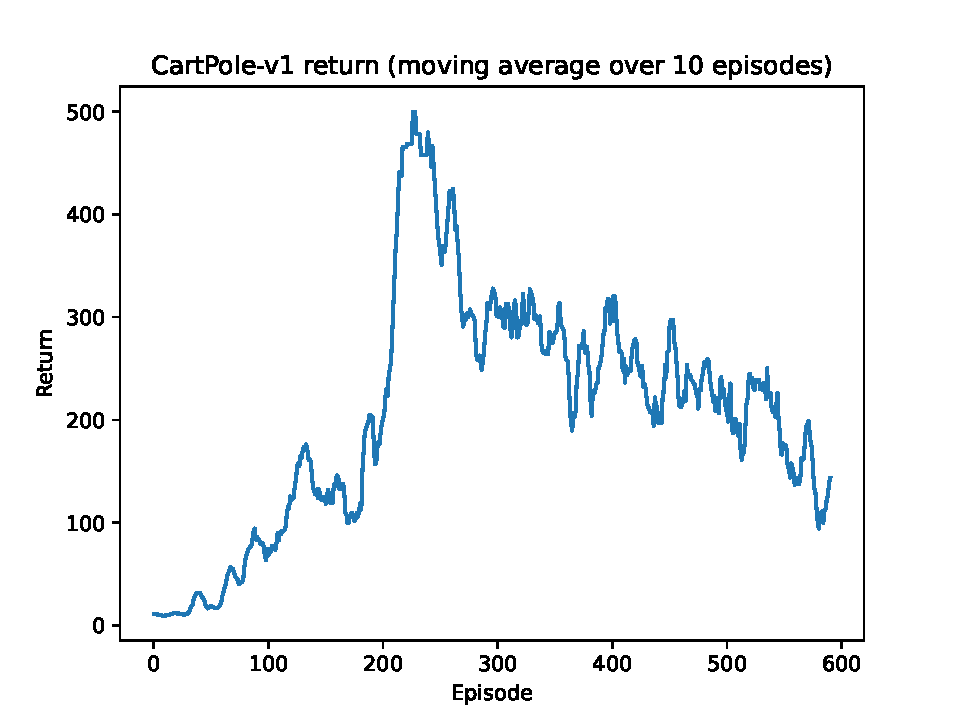
\includegraphics[width=\linewidth]{figures/cartpole/return_train_no_target_network.pdf}
    \caption{No target network}
  \end{subfigure}
  \begin{subfigure}{0.32\textwidth}
    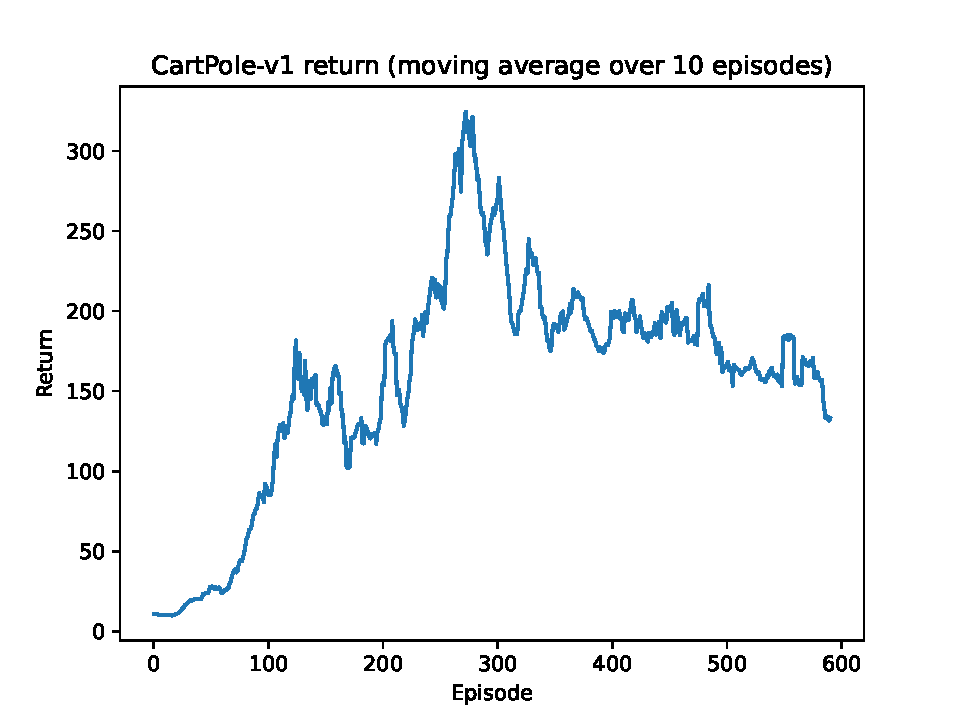
\includegraphics[width=\linewidth]{figures/cartpole/return_train_update_every_call.pdf}
    \caption{Update every call}
  \end{subfigure}
  \begin{subfigure}{0.32\textwidth}
    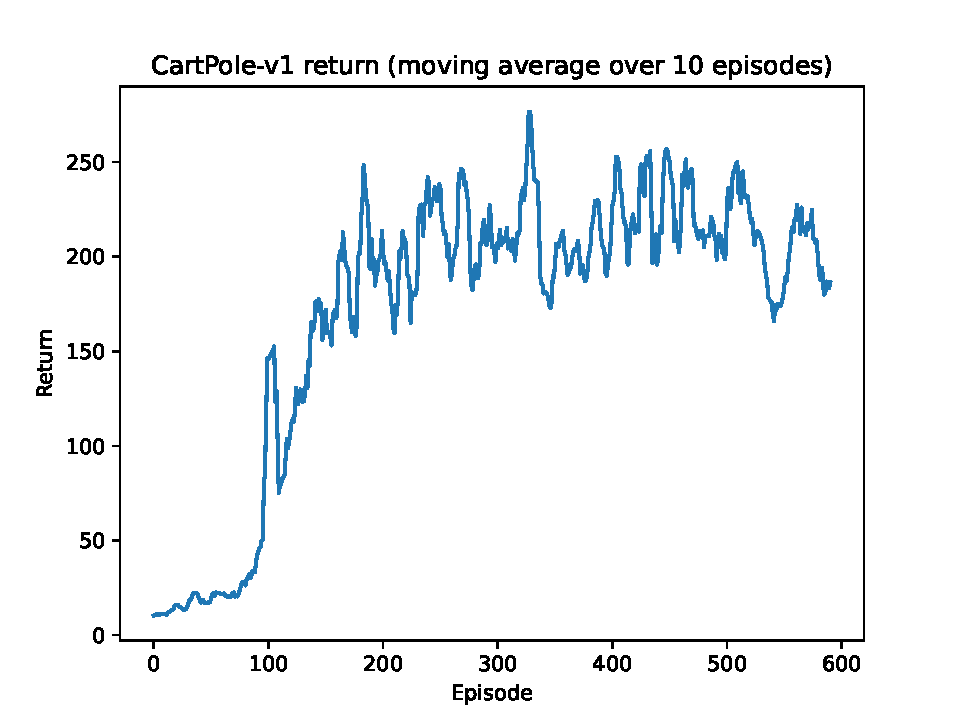
\includegraphics[width=\linewidth]{figures/cartpole/return_train_update_every_20_calls.pdf}
    \caption{Update every 20 calls}
  \end{subfigure}
  \caption{CartPole-v1: training return (running mean over 10 episodes).
  Without a target network the return reaches almost 500 around episode 230
  but then collapses. With a target network training is more stable.}
  \label{fig:cp-return}
\end{figure}

\begin{figure}[H]
  \centering
  \begin{subfigure}{0.32\textwidth}
    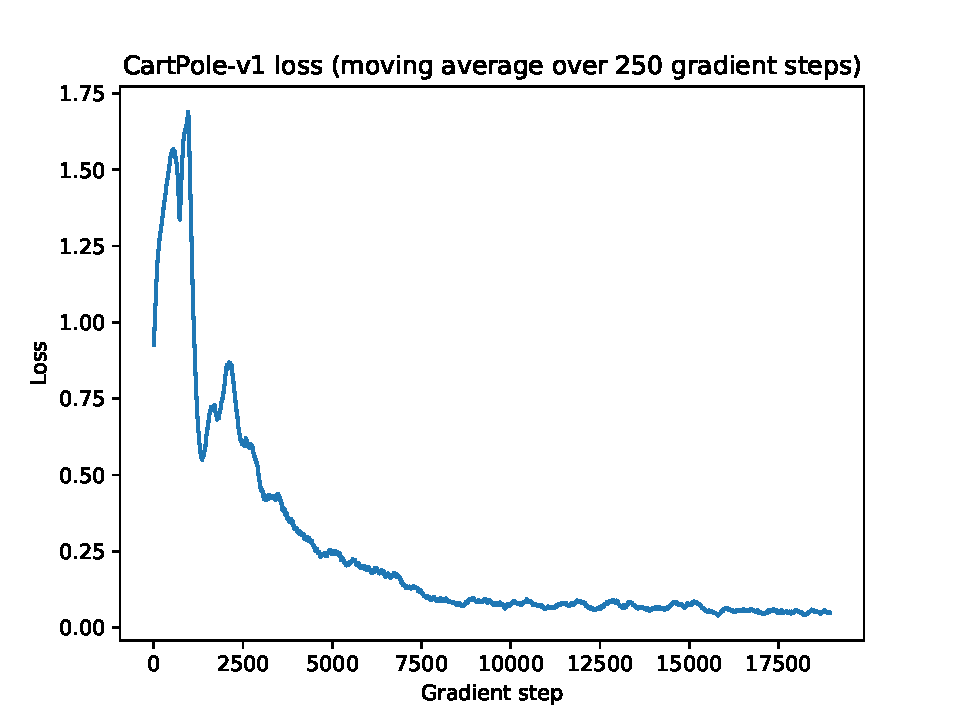
\includegraphics[width=\linewidth]{figures/cartpole/loss_train_no_target_network.pdf}
    \caption{No target network}
  \end{subfigure}
  \begin{subfigure}{0.32\textwidth}
    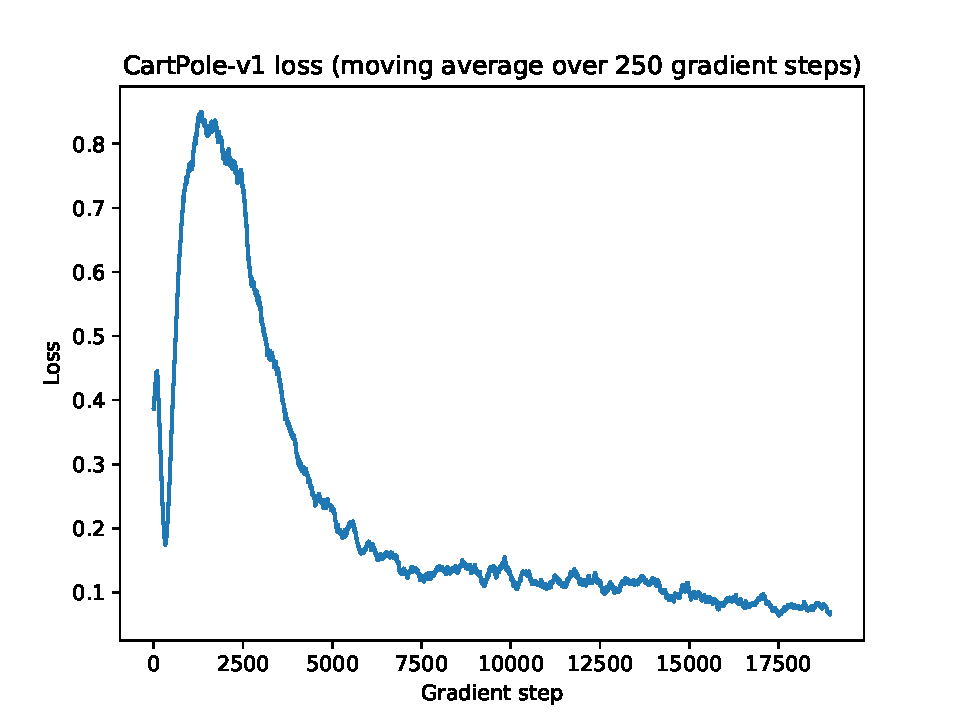
\includegraphics[width=\linewidth]{figures/cartpole/loss_train_update_every_call.pdf}
    \caption{Update every call}
  \end{subfigure}
  \begin{subfigure}{0.32\textwidth}
    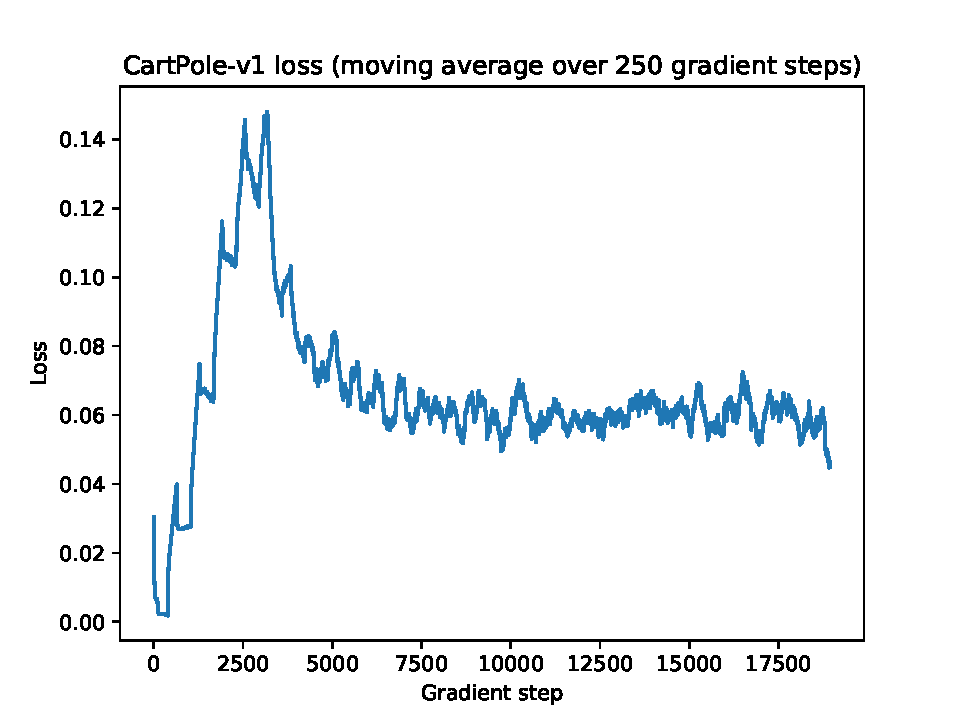
\includegraphics[width=\linewidth]{figures/cartpole/loss_train_update_every_20_calls.pdf}
    \caption{Update every 20 calls}
  \end{subfigure}
  \caption{CartPole-v1: training loss (running mean over 250 gradient steps).}
  \label{fig:cp-loss}
\end{figure}

\begin{figure}[H]
  \centering
  \begin{subfigure}{0.32\textwidth}
    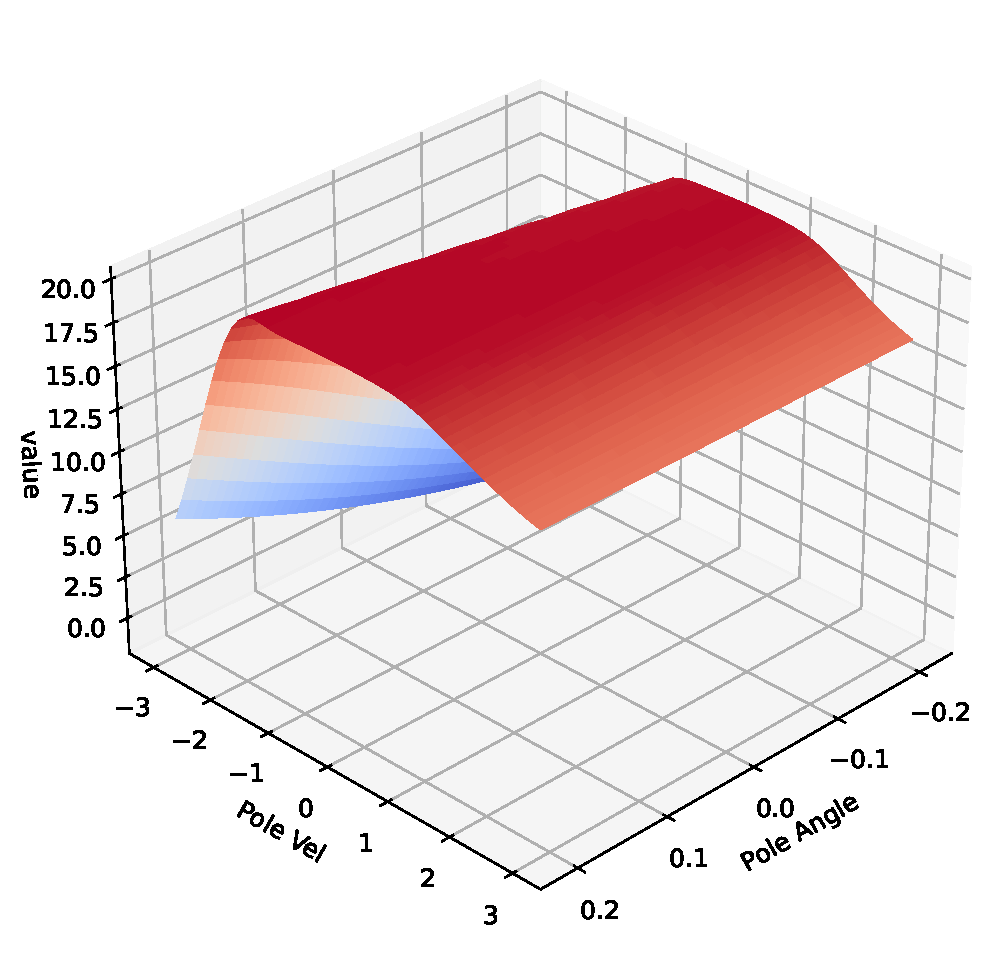
\includegraphics[width=\linewidth]{figures/cartpole/value_function_no_target_network_poleangle_polevel.pdf}
    \caption{No target network}
  \end{subfigure}
  \begin{subfigure}{0.32\textwidth}
    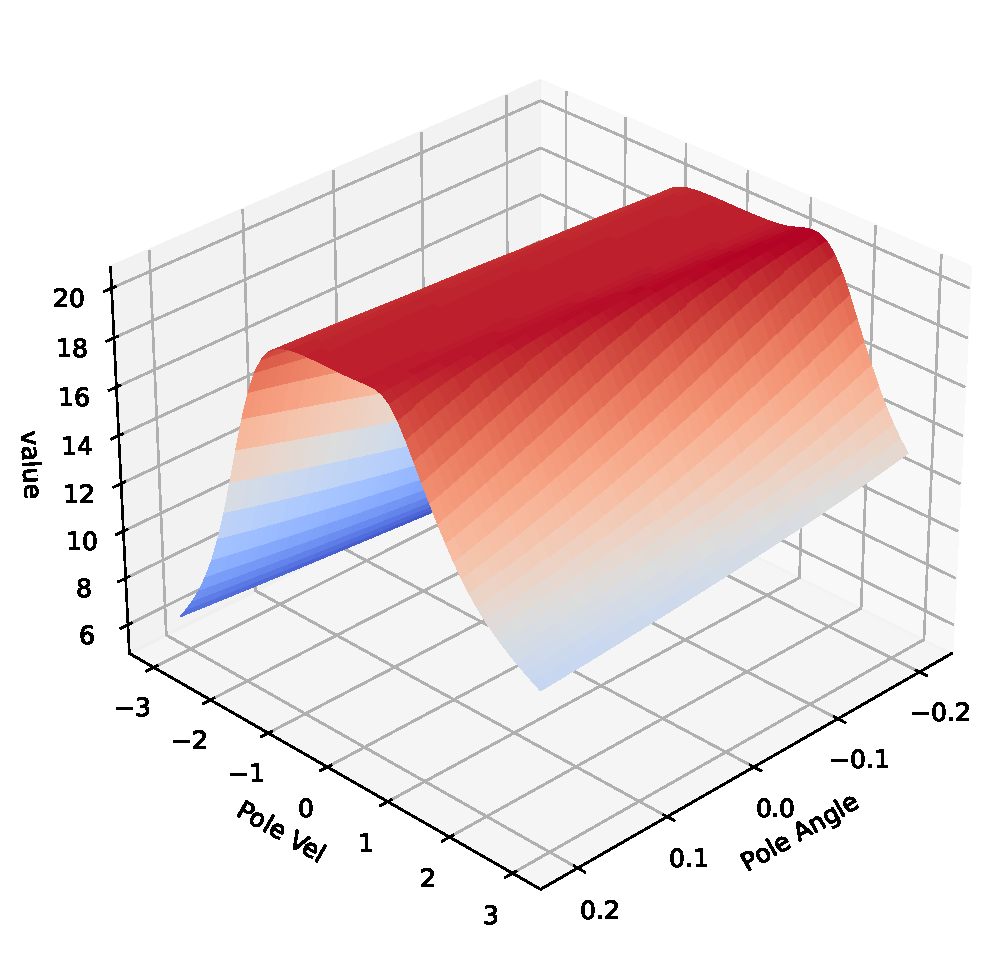
\includegraphics[width=\linewidth]{figures/cartpole/value_function_update_every_call_poleangle_polevel.pdf}
    \caption{Update every call}
  \end{subfigure}
  \begin{subfigure}{0.32\textwidth}
    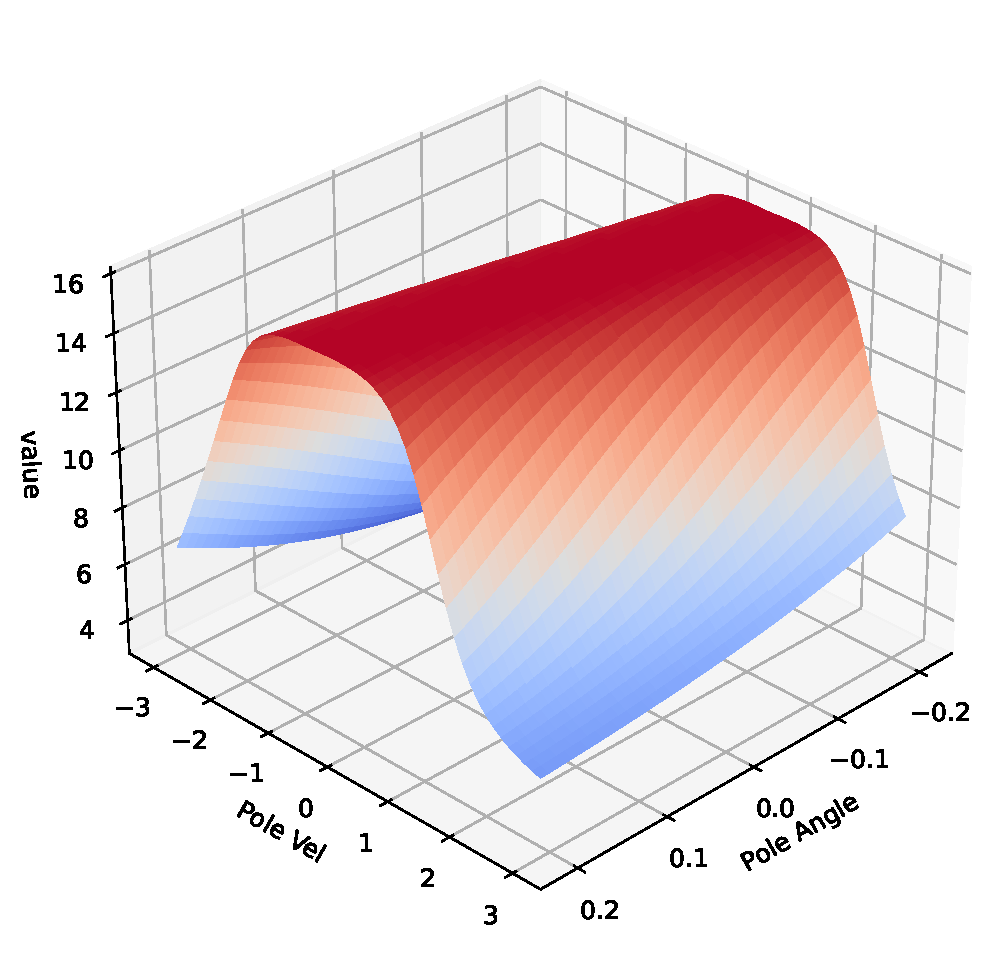
\includegraphics[width=\linewidth]{figures/cartpole/value_function_update_every_20_calls_poleangle_polevel.pdf}
    \caption{Update every 20 calls}
  \end{subfigure}
  \caption{CartPole-v1: $\max_a Q(s,a)$ over pole angle and pole angular
  velocity (cart position and velocity set to 0). The values level off at
  $1/(1-\gamma)=20$ where the pole can be balanced. They drop where the pole
  is already falling, i.e.\ angle and velocity have the same sign.}
  \label{fig:cp-value}
\end{figure}

\end{document}
